\section{Theoretical Framework}

\subsection{Reinforcement Learning}

Reinforcement Learning solves a particular kind of problem where decision-making is sequential, and the goal is long-term, such as game playing, robotics, resource management, or logistics \cite{100PML}. Reinforcement Learning is a computational approach to understanding and automating goal-directed learning and decision-making \cite{Sutton1998}. It is a subset of Machine Learning in which Intelligent Agents/Autonomous Agents take actions in an environment to complete a given task while aiming to maximize a numerical reward. This concept differs from that of Supervised and Unsupervised learning which together form the three paradigms of Machine Learning. Unlike the Supervised and Unsupervised Learning approaches, Reinforcement Learning is a more interactive approach, it does not have a fixed dataset whether it be labelled or unlabeled and rather uses a moving distribution of observations that results from the actions taken by the agent. This can be categorized as a closed-loop problem as the current actions influence the later inputs as this process repeats \cite{Sutton1998}. \\

\begin{figure}[h!]
    \centering
    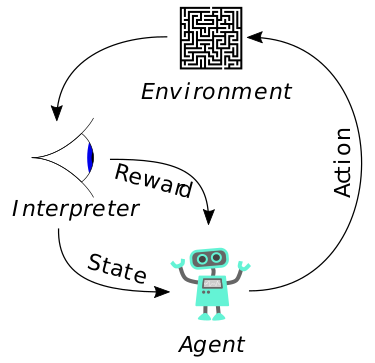
\includegraphics{images/Reinforcement_learning_diagram.svg.png}
    \caption{A simple Reinforcement Learning Scene \cite{wiki}.}
    \label{fig:RLD}
\end{figure}


\subsection{Components of Reinforcement Learning}

Figure \ref{fig:RLD} represents a simple scenario in Reinforcement Learning, where an Agent, which is tasked with achieving a goal in the given environment. The agent accomplishes this task by receiving observations from the environment and interacting with the environment by taking actions and receiving feedback from the environment for the actions taken. In the case of simple environments, the goal can be written directly in terms of a reward function that provide feedback to the agent for each state visited and each action taken, the agent tries to maximize this numerical reward by taking relevant actions and solving the task in the process. The agent here is known as the policy function, which maps the state-action pairs, and for a given state decides which action is appropriate that maximizes the reward. This state-action pair mapping can also be called the value function which determines the quality of the actions taken based on the feedback from the reward function. The aim here is to choose the best action for the given state to receive the highest possible reward. The policy function, value function, and reward function form the three main components of a Reinforcement Learning process that co-exist in a closed-loop system. This system can be modelled as a Markov Decision Process (MDP) \cite{Sutton1998} \cite{FMDP}, which is a discrete time based mathematical framework for modelling sequential decision making. This can be used to solve optimization problems by dynamic programming \cite{DPBE}. Sometimes Reinforcement Learning can include an extra element known as the Model of the environment. This is mentioned here as this too forms an integral part of certain categories of Reinforcement Learning but will not be elaborated in detail as it is out of scope for this research. This research is based on the Model-Free category of Reinforcement Learning. \\

\begin{figure}[h!]
    \centering
    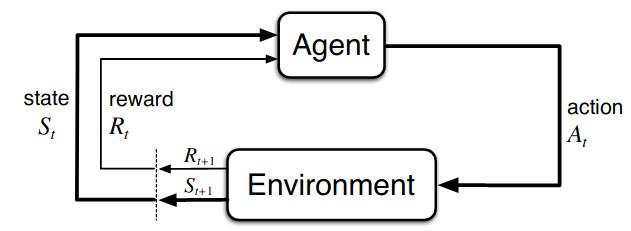
\includegraphics[width=\textwidth]{images/HMM.png}
    \caption{An agent interacting with the environment \cite{Sutton1998}.}
    \label{fig:HMM}
\end{figure}

The agent also known as the policy, usually denoted by $\pi$, is the decision-maker which means it specifies what action $A_t$ to take given a state $S_t$ at time $t$. More precisely $\pi$ gives the probability of an action or a probability distribution for different actions from which the best possible action for the given state is made. These actions are selected based on the reward it receives and the aim is to maximize this return. The expected return $G_t$ at given time $t$ can be formalized as per \ref{eq:1}. The environment here can either be episodic with a fixed number of time steps and a terminal state indicating the end of an episode, or continual which do not have any terminal state and never end. \\

\begin{equation}\label{eq:1}
    G_t = R_{t+1} + R_{t+2} + R_{t+3} + ... + R_T
\end{equation}

In these environments where the $T$ tends to infinity an additional term $\gamma$ also known as the discount factor is added to the above equation to induce simplicity and to prevent the expected returns from reaching infinity. Rewriting the expected returns including the discount factor results in equation \ref{eq:2}. \\

\begin{equation}\label{eq:2}
    G_t = R_{t+1} + \gamma R_{t+2} + \gamma^{2} R_{t+3} + ... + \sum_{k=0}^{\infty} \gamma^{k} R_{t+k+1}
\end{equation}

This discount factor usually has a value between 0 and 1, in most cases, this value tends to be closer to 1. \\

\subsection{V-Function \textit{vs} Q-Function}

The V-Function or state-value function, sometimes known as just Value Function, or simply $V$. This can be defined as the measurement of goodness for an agent to be in a particular state $S_t$ based on the returns $G_t$ following the current policy $\pi$. The value function is the expected total returns which can be discounted or undiscounted and can be expressed with equation \ref{eq:3}. \\

\begin{equation}\label{eq:3}
    V_{\pi} (s) = E_{\pi} [\sum_{k=0}^{T} \gamma^{k} R_{t+k+1} | s=s_t]
\end{equation}

Unlike the value function which defines a value for only the state, the Q-Function or action-value function, or simply $Q$, defines a value for each state-action pair. It can be quantified as a value of taking an action $A_t$ given a state $S_t$ at time $t$ following a policy $\pi$. The Q function can be written as $Q_{\pi} (s, a)$ and is the expected Return $G_t$ starting from $S_0$, after taking an action $A_0$, and then following a policy $\pi$ which can be expressed with equation \ref{eq:4}. \\

\begin{equation}\label{eq:4}
    Q_{\pi} (s, a) = E_{\pi} [\sum_{k=0}^{T} \gamma^{k} R_{t+k+1} | s=s_t, a=a_t]
\end{equation}

\subsection{Bellman Equation $\&$ Optimal Policy}

The Bellman Equation \cite{DPBE} \cite{BE} can be seen extensively in Reinforcement Learning related literature. The Bellman Equation expresses the relationship between the value of a state and the value of the successor states \cite{Sutton1998}. This can be broken down into two essential components the immediate reward and the discounted future rewards. In mathematical terms, the Bellman Equation can be defined by equation \ref{eq:5}. \\

\begin{equation}\label{eq:5}
    V(s) = E [R_{t+1} + \gamma V(S_{t+1}) | S_t = s]
\end{equation}

Based on this general form of the Bellman Equation it can be rewritten to suit both the V-Function and Q-Function as shown by equations \ref{eq:6} and \ref{eq:7}. These equations express the relationship between the value of the state and the value of its successor states. \\

\begin{equation}\label{eq:6}
    V_{\pi}(s) = \sum_{a} \pi (a|s)\sum_{s^{'}} P(s^{'}|s) [R(s, a) + \gamma V_{\pi} (s^{'})]
\end{equation}

\begin{equation}\label{eq:7}
    Q_{\pi} (s, a) = \sum_{s^{'}} P(s^{'}|s, a)[R(s, a) + \gamma\sum_{a^{'}} \pi (a^{'}|s^{'}) * Q_{\pi} (s^{'}, a^{'})] 
\end{equation}

Any policy which can maximize a total cumulative reward can be classified as an optimal policy, represented as $\pi *$. For Finite Markov Decision Processes, an optimal policy exists but may not be unique, meaning there could be different optimal policies sharing a common value function known as optimum value function which can be defined as the function which yields the maximum value, represented by equation \ref{eq:8}. Similar is the case for an optimal action-value function, represented by equation \ref{eq:9}. \\

\begin{equation}\label{eq:8}
    V_{*} (s) = max_{\pi} V_{\pi} (s) 
\end{equation}

\begin{equation}\label{eq:9}
    Q_{*} (s, a) = max_{\pi} Q_{\pi} (s, a)
\end{equation}

Equation \ref{eq:8} and \ref{eq:9} represents the optimal state value function and action-value function which can be further combined with the Bellman Equation to get the Bellman Equation of Optimality as shown by equation \ref{eq:10} and \ref{eq:11} for the state value function and the action-value function respectively. Bellman optimality equation expresses the fact that the value of a state under an optimal policy must equal the expected return for the best action from that state \cite{Sutton1998}. \\

\begin{equation}\label{eq:10}
    V_{*} (s) = max_{a} \sum_{s^{'}} P(s^{'}|s)[R(s, a) + \gamma V_{*} (s^{'})]
\end{equation}

\begin{equation}\label{eq:11}
    Q_{*} (s, a) = \sum_{s^{'}} P(s^{'}|s, a)[R(s, a) + \gamma max_{a^{'}} Q_{*} (s^{'}, a^{'})]
\end{equation}

\subsection{On-Policy \textit{vs} Off-Policy}

The main objective of both types of learning is to evaluate a Q-function $Q(s, a)$ to predict cumulative future discounted rewards given a state $S$ and action $A$. \\ 

In on-policy learning, the $Q(s,a)$ function is learned from actions that are taken using the current policy $\pi(a|s)$. An example of on-policy learning is the SARSA algorithm \cite{zou2019finitesample}. The update rule for the SARSA algorithm as per the Bellman Equation can be written as per equation \ref{eq:12}, where the action $a^{'}$ is taken as per current policy $\pi$. \\

\begin{equation}\label{eq:12}
    Q(s, a) = Q(s, a) + \alpha [r + \gamma Q(s^{'}, a^{'}) - Q(s, a)]
\end{equation}

Comparing this to the off-policy learning, $Q(s, a)$ function is learned from taking different actions including random actions without even the need to define a policy. An example of off-policy learning is the Q-Learning algorithm \cite{QL} where an optimal policy can be reached using random actions for exploration without specifying a policy before learning. The update rule for the Q-learning algorithm as per the Bellman Equation can be written as per equation \ref{eq:13}, where $a^{'}$ are all the actions that were taken in-state $s^{'}$. \\

\begin{equation}\label{eq:13}
    Q(s, a) = Q(s, a) + \alpha [r + \gamma max_{a^{'}} Q(s^{'}, a^{'}) - Q(s, a)]
\end{equation}

The research in this paper is based on the off-policy style of learning algorithms and the related concepts will be briefed in the following sections. \\

\subsection{Q-Learning}

\begin{figure}[h!]
    \centering
    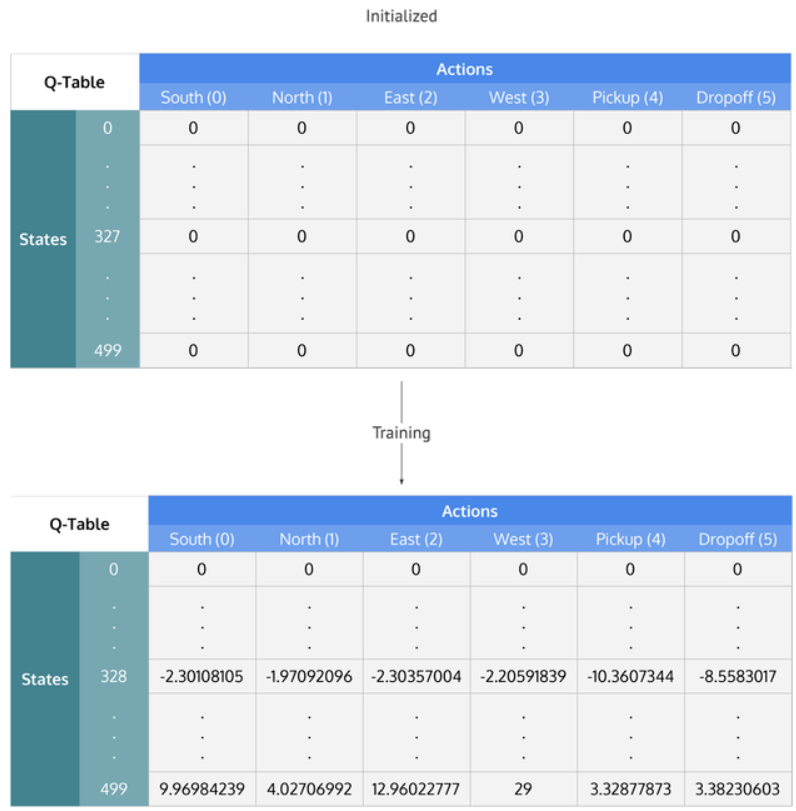
\includegraphics[width=\textwidth]{images/Q-Table.png}
    \caption{A simple example of a Q-Table \cite{wiki}.}
    \label{fig:QT}
\end{figure}

The Q-Learning algorithm \cite{QL} was one of the earliest Reinforcement Learning algorithms proposed in 1989, which even to date is being used in some form. Equation \ref{eq:13} shows the Bellman update rule for the algorithm, where $\alpha$ is the learning rate that controls the convergence rate. The learning rate usually has a value between 0 and 1. \\

Q-Learning is an off-policy Reinforcement Learning algorithm that evaluates an action-value function Q(s, a) to find the optimal action-value function $Q^{*}$. Q-Learning uses a table-based storage system known as Q-Table to store and later look up the Q values for each state-action pair. As the agent explores the environment and makes actions, the Q values are determined using the update equation, and the combination of (Q-value, State, Action) are stored in the Q-Table. Each pair combination of the state and action will have a corresponding Q-value and will be constantly updated using the update rule. Figure \ref{fig:QT} shows a simple Q-Table containing 6 actions and 500 states and the corresponding Q-value for each state-action pair. \\

The Q-Learning algorithm has shown great success by solving many tasks in Reinforcement Learning. But this kind of brute force method has a severe problem. For example in cases where the state space and action space are orders of magnitude higher, storing each and every value and then dynamically searching and updating increases the computation time and hardware resources making this computationally too expensive for simpler tasks. Here is where the generalization capabilities of Artificial Neural Networks \cite{mcculloch1943logical} can be leveraged, instead of storing and updating each and every Q-value, given the state as the input the Q-value can be approximated by a neural network for the set of actions, from which the best action for a given state can be selected. \\

\subsection{Neural Network Function Approximation $\&$ Deep Q-Learning}

\begin{figure}[h!]
    \centering
    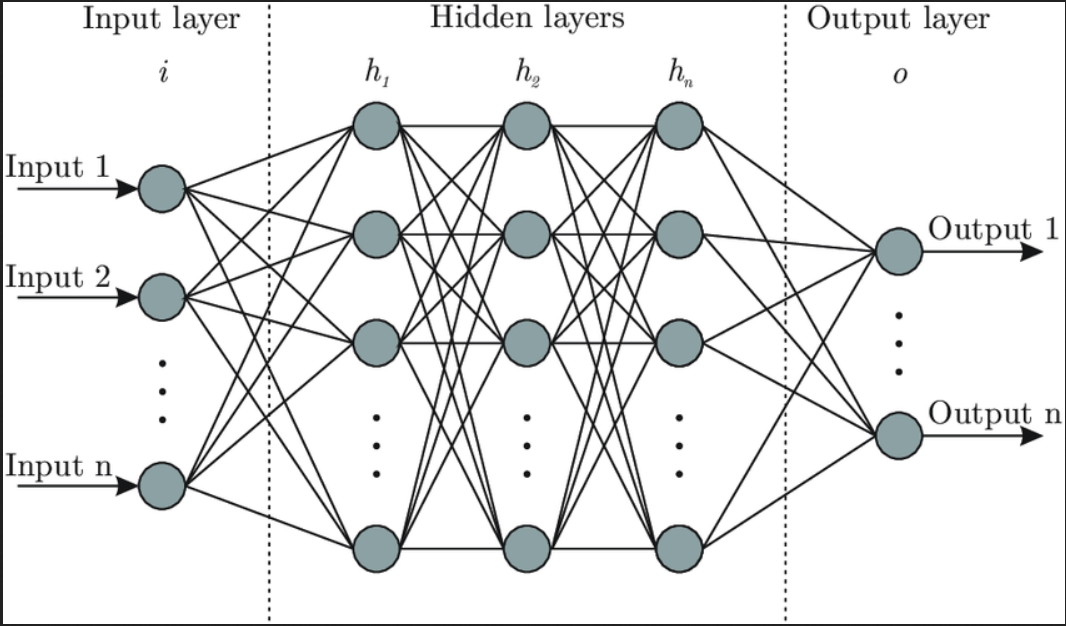
\includegraphics[width=\textwidth]{images/ANN.png}
    \caption{A simple representation of a Neural Network \cite{ANNPic}.}
    \label{fig:ANN}
\end{figure}

Figure \ref{fig:ANN} shows a pictorial representation of a simple Artificial Neural Network (ANN) also known as a Multi-Layer Perceptron in technical terms, derived and developed from the original Rosenblatt Perceptron Model \cite{rosenblatt1958perceptron}. Extensive research has been conducted in this field of deep learning by the likes of Geoffrey Hinton, Yoshua Bengio, Yann LeCun, Ian Goodfellow, Andrew Ng and this research follows and refers to such works. These researchers have covered topics on this field extensively and it will not be detailed elaborately here as it is out of scope for this research. However, basic related concepts will be briefed. \\

The general theory behind a perceptron is, N amount of features is connected to the M amount of outputs with the help of W amount of weights and the strength of these weights between these connections determines the relation between the input and output. In this manner, the input can be mapped to the output by changing or updating the weights. The individual unit in the perceptron is called a neuron, named after the biological neurons present in the nervous system. These neurons take input and after applying a degree of non-linearity give an output, mathematically this can be represented by equation \ref{eq:14}. \\

\begin{equation}\label{eq:14}
    Y_k = \textit{f} [W_{jk} * X_k + B]
\end{equation}

X represents the value of the neuron usually the input, W is the weight of the connection usually initialized with random values, B is a value of bias that is added to every operation and Y is the output after the application of a certain degree of non-linearity. The combination of multiple of these perceptron's to form layers, both horizontally and vertically as represented in figure \ref{fig:ANN} is a multi-layered perceptron, but the basic principle remains the same. By updating these weights the relation between a given input and output can be approximated successfully. Most modern neural networks update their weights by using a technique known as backpropagation \cite{kelley1960gradient}, which can be defined as a gradient descent method to minimize a cost or loss function. This loss function can be defined as per the given problem, an example of a simple loss function is shown in equation \ref{eq:15}. \\

\begin{equation}\label{eq:15}
    MSE = \frac{1}{n} \sum_{i}^{n} (Y_i - Y_i^{'})^2
\end{equation}

To minimize this loss function, the weights can be updated using the weight update equation from the stochastic gradient descent \cite{ruder2016overview} to approximate a function. Immediately this can be seen as a much efficient way when compared to storing values in a lookup table for every input-output pair as discussed in the previous section regarding Q-Learning. Deep Q-Learning (DQN) \cite{mnih2013playing} leverages this power of ANN's to efficiently approximate the Q-values for the state-action pairs. The principle of Deep Q-learning remains the same for the most part, but this eliminates the need for a computationally heavy lookup table and instead uses ANN to predict the Q-values for each action, and for a given state the action with the highest Q-value is chosen as the most probable action at that given time step. \\

\subsection{Double Deep Q-Learning}

As per the Mean Squared Bellman Error Equation, there is a Q-value and a Target Q-value, the error between these values is calculated as the output of the loss function which is then used to update the weights of the network using gradient descent. In DQN both the Q-value and the target Q-value are estimated by a single network in many cases resulting in something called overestimation bias. This means that as the training progresses as the same network is used to estimate two moving values based on maximum returns, it sometimes tends to return higher values for the actions which may not be the best possible choice for that given state. \\

To solve this problem a simple trick was set up, instead of one, two networks were proposed leading to the algorithm called Double Deep Q-Learning (DDQN) \cite{vanhasselt2015deep}. Here there are two copies of the same network, the one estimating the Q-value and the other estimating the Q-target. Q-target remains stationary and is updated every few time steps by copying the weights from the first network. This enables more stable updates without the problem of overestimation. \\

\subsection{Actor Critic Methods}

\begin{figure}[h!]
    \centering
    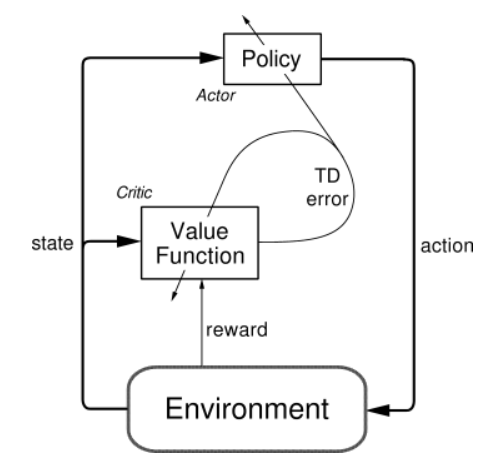
\includegraphics[width=\textwidth]{images/AC.png}
    \caption{Actor Critic Architecture \cite{Konda00actor-criticalgorithms}.}
    \label{fig:AC}
\end{figure}

Policy Gradient \cite{PG} methods are on-policy learning algorithms that target modeling and optimizing a policy directly, unlike Q-learning which does not require a policy to be specified. Temporal Difference \cite{TD} is a technique to predict the expected value given a sequence of states, which acts as a base for most model-free Reinforcement Learning algorithms. Actor-Critic \cite{Konda00actor-criticalgorithms} algorithms are a different class of Reinforcement Learning algorithms but with the same goal which is to find an optimal behaviour strategy that returns maximum rewards.  Simply put Actor-Critic is a Temporal Difference version of Policy Gradient. Another difference between Actor-Critic and Q-Learning is, DQN uses one network to estimate the Q-values of the actions, Actor-Critic use two individual networks one for the Actor and the other for the critic. In DQN for a given state, the network estimates Q-values for all the probable actions, and the action with the highest Q-value is chosen as the best possible action for that given state, in Actor-Critic, the Actor chooses the action for the given state, and the critic evaluates this action by estimating a value function and tells the actor how good the current action is and how to update it further. The actor-network is updated based on the critic value and the critic network is updated by using the actor's actions, both work in tandem and are updated dynamically. This paper will not dive deep into this class of Reinforcement Learning as this is out of scope for this research, but a summary was provided just as an introduction because this is an important concept that will be used as a backbone for other algorithms used extensively in this paper. \\

\subsection{Deep Deterministic Policy Gradients}

DQN style algorithms work well and are more suited for deterministic actions spaces. Deterministic actions spaces have a fixed number of actions, for example, Left, Right, Up, Down. Continuous action spaces as the name suggests have continuous values, for example, any value in the coordinate system. It is not possible to straightforwardly apply Q-learning to continuous action spaces, because in continuous spaces finding the greedy policy requires optimization of actions at every time step, this optimization is too slow to be practical with large, unconstrained function approximators and nontrivial action spaces \cite{lillicrap2019continuous}. A continuous action space can be discretized, but the resulting high number of actions is another limitation that DQN cannot solve. This led to the need for a new class of algorithms able to handle high dimensional continuous action spaces. Research in this area led to a combination of Q-Learning style of learning with the Actor-Critic based algorithms which resulted in the Deterministic class of Reinforcement Learning algorithms of which one of the main algorithms is Deep Deterministic Policy Gradient (DDPG) \cite{lillicrap2019continuous}. \\

DDPG is an off-policy deterministic algorithm which means it returns actions deterministically rather than stochastically \cite{haarnoja2018soft}. The output of a DQN algorithm is probabilistic, which is the highest probability of an action given a particular state, DDPG outputs the exact values of the actions for that given state. DDPG also use an Actor-Critic based architecture, here the actor-network is a policy gradient that takes in states as the inputs and outputs the exact continuous values as actions, the critic-network is a Q-Value network that takes the states and actions as inputs and outputs the corresponding Q-values. The architecture of a DDPG algorithm is designed in such a way that it contains two Actor Networks, a current actor and a target actor, and two Critic Networks, a current critic and a target critic. Both the Current Actor and Critic Networks have their loss functions to minimize during the learning process and the updated weights of the Current Networks are copied onto the target networks. All the four networks are involved during the training process in updating the weights which can be seen from equations \ref{eq:16} and \ref{eq:17}. After the training process is complete only the Actor-Network with the optimal policy can be used for inference. \\

\begin{equation}\label{eq:16}
    J_{Q} = \frac{1}{N} \sum_{i}^{N} [R_i + \gamma (1 - T) Q_{target} (S_{i}^{'}, \mu_{target} (s_{i}^{'})) - Q (s_i, \mu (s_{i}))^2 ]
\end{equation}

\begin{equation}\label{eq:17}
    J_\mu = \frac{1}{N} \sum_{i}^{N} Q(s_i, \mu(s_i ))
\end{equation}

Equation \ref{eq:16} is the critic networks loss function for estimating the Q-values. This loss is very similar to the mean squared bellman loss and it uses both the advancements from the DQN and DDQN algorithms. Here is where the current and target networks come into play in the DDPG algorithm. The current network estimates Q-values for the current states and actions, whereas the target network estimates the Q-values for the next states and the target actions, these target actions coming from the actor target predictions. Equation \ref{eq:17} is the Actor loss which is simply the sum of all the Q-values which the goal is to maximize the result so as the have higher Q-values. Compared to DDQN which performs a hard update by directly copying the weights of the main network to the target network, the new changes introduced here are to perform a soft update instead. Due to dynamic updates and moving Q-values, this provides further stability during the updates which results in faster convergence for the algorithm even in complex environments. The update equations for the target networks are given by Equation \ref{eq:18} and \ref{eq:19}. \\

\begin{equation}\label{eq:18}
    \theta^\mu_{target} = \tau \theta^\mu_{target} + (1 - \tau)\theta^\mu
\end{equation}

\begin{equation}\label{eq:19}
    \theta^Q_{target} = \tau \theta^Q_{target} + (1 - \tau)\theta^Q
\end{equation}

Here $\tau$ is the parameter that controls the degree to which the parameters are copied during the soft update, this value usually lies between 0 and 1, and is typically chosen closer to 1. \\

\subsection{Twin Delayed Deep Deterministic Policy Gradients}

DDPG has shown great success in many complex tasks and even solving robotics tasks which is the essence of this research. It has also been used as the base algorithm for many other successful related research. While it can achieve great performance it can also be brittle sometimes concerning hyperparameters and takes longer to converge, resulting in higher training and tuning times. One of the main failures of DDPG is the Q-Network's overestimation of the Q-values. This overestimation leads to the higher Q-values for actions that may not be suitable for the given state, and when the actor learns from these Q-values the policy beings to break or diverge to some unsuitable behaviour. \\

To fix these issues and improve the performance of the baseline DDPG algorithm, a new method called the Twin Delayed Deep Deterministic Policy Gradients (TD3) \cite{fujimoto2018addressing} was proposed. TD3 aims to address a few of the shortcomings of DDPG by using three new implementations. First, Clipped Double Q-Learning, TD3 uses two Q-Networks unlike DDPG which uses one and uses the smaller of the two estimated Q-values in the mean squared bellman equation, this is a simple and intuitive method of reducing the overestimation bias of the Q-values. Second, Delayed Policy and Target updates, along with the soft update rule the TD3 algorithm updates both the Actor Networks and the target networks in a delayed manner. As per the paper, the Actor and the Target Networks are updated once every two Q-Network updates. This manner of updates allows the actor to see better Q-values along with improved stability leading to robust learning and faster convergence. Third, Target Policy Smoothing, TD3 adds some noise to the target actions, which is the output of the target actor-network, this is to make it harder for the policy to exploit Q-function errors by smoothing out Q-values \cite{fujimoto2018addressing}. Together these improvements result in sustained and improved performance, better stability and faster convergence when compared to DDPG and TD3 will be used and the base algorithm in this research. \\

\subsection{Experience Replay Memory}

The involvement of neural networks in combination with off-policy Reinforcement Learning has shown great success and one of the important reasons is the use of Experience Replay \cite{zhang2018deeper} \cite{fedus2020revisiting}. This is a simple method that enables the agent to save data as it interacts with the environment. The usual format of saving data is $(S_t, A_t, R_{t+1}, S_{t+1})$, Current State, Current Action, Reward, Next State. The recent versions of the experience replays include an additional term that specifies the end of an episode known as the terminal state. This flag is useful in determining whether or not to calculate the discounted future rewards. The data is stored in this format in the memory continuously on a first in first out basis. For learning the agent can randomly sample a mini-batch from the memory and use this to update its weights. This random sampling of a mini-batch from the memory is highly advantageous by introducing a degree of variance as consecutive examples in a Reinforcement Learning environment are highly temporally correlated, and gradient descent methods do not perform well with correlated data. \\

There have been many recent advances with experience replay, namely Prioritized Experience Replay (PER) \cite{schaul2016prioritized} which changes the way how data is presented to the agent emphasizing on data with greater TD error which has shown to speed up training, Hindsight Experience Replay (HER) \cite{andrychowicz2018hindsight} taking advantage of the replay memory to augment the data with new rewards in a sparse reward system where the agent does not get to see positive feedback and in the process accelerates training. The research is this paper does not use any advanced version of experience replay and just uses two replay buffers instead which will be explained in detail in the methods section. \\

\subsection{Hindsight Experience Replay}

\begin{figure}[h!]
    \centering
    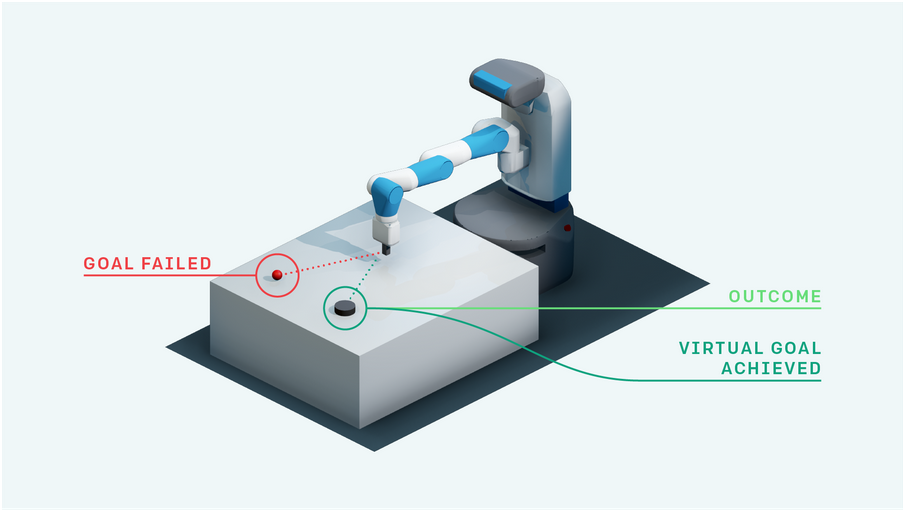
\includegraphics[width=\textwidth]{images/HER.png}
    \caption{Example of Hindsight Experience Replay \cite{andrychowicz2018hindsight} \cite{plappert2018multigoal}.}
    \label{fig:HER}
\end{figure}

HER provides a very intuitive solution by taking advantage of the off-policy replay memory trick by augmenting new data into the already present data in the memory. Such a system is highly useful in environments where the reward is sparse. Sparse reward environments provide almost no information to the agent during the initial phase of learning. Traditionally the agent takes a very long time to see any positive reward hence resulting in large training times. As sparse reward environments are goal-based environments, HER augments the data by providing a positive reward to the achieved goals even though they might be failed instances with the actual goal still to be reached. For example, when the agent in a walking simulator has to reach a particular destination of 100m in the environment but ended up falling short by 20m, the episode has ended and the agent has not reached its main goal. But, what HER does here is it uses the already reached goal of 80m and other similar instances and provides it with a positive reward, the original reward from the environment being negative. By providing positive feedback sooner in the form of virtual goals the agent can see more rewards and in the process eventually end up reaching the desired goal as seen by a simple representation in figure \ref{fig:HER}. This process has shown great success in sparse reward environments and solving complex robotics tasks \cite{plappert2018multigoal}. There are different strategies used for such data augmentation like randomly assigning failed instances as virtual goals, using the end of the episode as virtual goals, or using a distance-based method \cite{HERER} to assign virtual goals to achieve the original goal faster, further accelerating the training in such environments. \\

\subsection{Exploration Exploitation Dilemma}

\begin{figure}[h!]
    \centering
    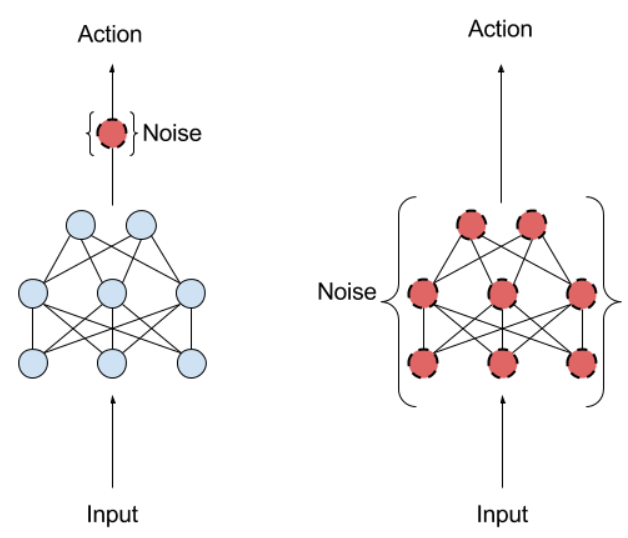
\includegraphics[width=\textwidth]{images/ANPN.png}
    \caption{Difference Between Action Noise and Parameter Noise \cite{plappert2018parameter}.}
    \label{fig:ANPN}
\end{figure}

All Reinforcement Learning algorithms have to go through two important phases during the training process, the exploration phase and the exploitation phase. To maximize the returns the agent needs to learn from the past actions which were desirable and repeat those actions to increase the cumulative reward, this process is known as exploitation. But, to select the best actions the agent needs to perform different actions and receive feedback from the environment to determine which of these actions are the best. The trade-off between exploration and exploitation is known as The Exploration-Exploitation Dilemma which has been an active area of research in Reinforcement Learning for many years. \\

One fairly common approach is called the Epsilon-Greedy or $\epsilon$-Greedy Strategy. In this strategy, the agent starts by taking random actions to explore the different states. The $\epsilon$ parameter controls the degree to which the agent takes random or greedy actions. Actions from the agent are known as greedy actions. Over the course of training the $\epsilon$ starts which a high value making the agent take random actions and then the value of $\epsilon$ is reduced and the agent transitions from taking random actions to greedy actions. This way the agent first starts with exploring the environment then goes to exploiting in the later stages of training and a balance between exploration and exploitation is achieved. The $\epsilon$ value is not made entirely zero as even during the exploitation phase some amount of random exploration is desired, and the rate of decrement of this $\epsilon$ value can be controlled as per requirement. \\

This strategy is highly used in Q-Learning related algorithms. The more deterministic algorithms like DDPG and TD3 use noise-based exploration strategies. Noise is induced in some form associated with the actions and this way the agent explores the environment. The network is trained with the noise and learns this noise during the exploitation phase resulting in more robust policies. Two types of noise can be added as seen in figure \ref{fig:ANPN}, one is the action noise \cite{lillicrap2019continuous} \cite{fujimoto2018addressing}, where the noise is directly added to the output actions of the actor-network, the second is the parameter noise \cite{plappert2018parameter}, where noise is added to the weights of the actor-network resulting in perturbed actions. \\

Exploration is an important part of Reinforcement Learning as, without exploration, exploitation is not possible and also does not make sense. For complex environments like robotics, the exploration becomes difficult and this phase takes a major part of the training time to explore the high dimensional state spaces to efficiently exploit the good actions. To accelerate Reinforcement Learning some strategies need to be used to overcome this exploration phase like curiosity-driven exploration with intrinsic rewards \cite{burda2018exploration}, multi-agent exploration \cite{lowe2020multiagent}, the combination of both \cite{lanier2019curiositydriven}, or by leveraging the power of demonstrations which is an important area of focus for this research. \\

\subsection{Reward Engineering}

\begin{figure}[h!]
    \centering
    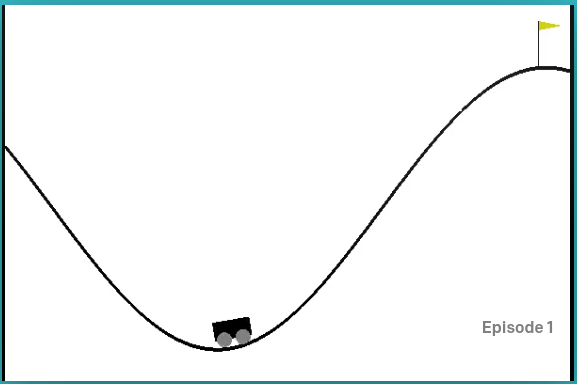
\includegraphics[width=\textwidth]{images/MC.png}
    \caption{Open AI Gym Simple Mountain Car Environment \cite{brockman2016openai}. }
    \label{fig:MC}
\end{figure}

A reward function is one of the three basic components of Reinforcement Learning. As mentioned in the earlier parts of the literature a Reinforcement Learning agent aims to maximize the rewards to ultimately reach an optimal policy. This makes the design of the reward function as important as the design of the policy or the algorithm because the reward function has the power to control the training of the agent. Figure \ref{fig:MC} shows the example of a simple mountain car environment where the reward can be designed in terms of the distance to the flag and velocity of the vehicle as well, but a simple distance reward will do well in this case. A Reinforcement Learning algorithm can directly optimize this reward to reach a good policy. In complex environments which high dynamics such as robotics, a straightforward metric based reward function is not possible due to the involvement of complex interactions. This raises a need for research into reward design for complex environments. The trade-off here is, a simple reward design may not be as effective in enabling the agent in reaching an optimal solution, while a well-engineered reward function may lead to sub-optimal policies. The reward function also plays a major role in the exploration-exploitation phases of the agent, so there is a need to design an optimal reward function balancing the exploration and exploitation, by providing the correct information to the agent, so that it can learn efficiently. Previous research "Reward Engineering for Object Pick and Place Training" \cite{nagpal2020reward} has found success in this area of reward engineering for complex robotics tasks and using that as motivation this area will be an important focus for this research. One of the aims of this research is to design a simple and effective reward function that can provide fast and robust learning. \\

\subsection{Imitation Learning $\&$ Behavior Cloning}

The two main areas of research related to decision making in autonomous robots in recent times are Reinforcement Learning and imitation learning. The basic idea of imitation learning, sometimes known as learning from demonstrations, is that the learning agent receives examples on how to perform actions from an expert demonstrator, and the agent mimics these actions to try and replicate the expert's behaviours. Humans widely use a similar form of learning by referring to experts and trying to mimic those actions as well as retrying similar actions themselves to solve a particular task. The main focus of this research is to try and combine both to solve complex tasks. \\

The simplest and most common form of imitation learning among many others is Behaviour Cloning which uses a supervised learning approach to train an agent. There is a dataset of expert demonstrations in the form of state-action pairs and the agent is trained by minimizing a loss function that estimates the error between the agent's actions and the expert's actions for the given states. A simple Behaviour Cloning loss function can be written like equation \ref{eq:20}. \\

\begin{equation}\label{eq:20}
    BC_{loss} = \frac{1}{n} \sum_{i}^{n} (A_{expert} - A_{agent})^2
\end{equation}

Behaviour Cloning has shown success in many areas solving complex tasks like self-driving \cite{bojarski2016end}, drone navigation \cite{QN}, biped locomotion \cite{BL}, but struggles with generalization outside the demonstration data. Plain Behaviour Cloning heavily relies on the quality and quantity of demonstrations and either perform well for certain tasks or other tasks, worse than a random agent sometimes resulting in undesirable behaviours. Several techniques help with data augmentation and expert data but they constantly rely on the expert being present even during training and cannot do with just a pre-collected dataset. \\

\subsection{Behavior Cloning $\&$ Reinforcement Learning}

Some of the drawbacks of Behaviour Cloning can be solved by combining it with Reinforcement Learning. Previous work has been successful in doing so, demonstrations have been used to speed up learning in simple environments such as cart-pole \cite{RLFD}. Recent works have shown great success in this front by managing to solve complex multi-goal robotics tasks \cite{nair2018overcoming}. This research is very closely related to two recent works combining Behaviour Cloning and Reinforcement Learning, "Overcoming Exploration in Reinforcement Learning with Demonstrations" \cite{nair2018overcoming} and "Integrating Behavior Cloning and Reinforcement Learning for Improved Performance in Dense and Sparse Reward Environments" \cite{goecks2020integrating}. This research aims to accelerate Reinforcement Learning for complex multi-goal robotics environments by leveraging demonstrations. Previous research has shown success in the same tasks but it either comes in the form of complex implementations or the use of heavy computing resources. \\